\documentclass [12pt,twoside]{article}
\usepackage[utf8]{inputenc}
\usepackage[T1]{fontenc}

%Page margins, header and footer positions
\usepackage{geometry}
\geometry{
    a4paper,
    total={210mm,297mm},
    left=25mm,
    right=25mm,
    top=30mm,
    bottom=25mm,
    headsep=7mm}

\interfootnotelinepenalty=10000

%To display filling dots in the TOC for all entries
\usepackage[titles]{tocloft}
\renewcommand{\cftsecleader}{\cftdotfill{\cftdotsep}}

%Define new header and footer style
\usepackage{fancyhdr}

\pagestyle{fancy}
\fancyhf{}
\lhead{\color{Gray}{\small{CLup project by Davide Luca Merli, Dario Passarello}}}
\lfoot{\textcolor{Gray}{\small{Copyright © 2020, Davide Luca Merli, Dario Passarello – All rights reserved}}}
\rfoot{\textcolor{Gray}{\thepage}}
\renewcommand{\headrulewidth}{0pt}

%PACKAGES
\usepackage{wasysym}
\usepackage{pifont}

\newcommand{\supported}{\ding{52}\xspace}
\newcommand{\unsupported}{\ding{55}\xspace}
\newcommand{\partsupported}{\textcolor{black!40}{\ding{52}}\xspace}
\newcommand{\lowsupported}{\textcolor{black!20}{\ding{52}}\xspace}
\newcommand{\unknowsupported}{\textbf{?}\xspace}

%Font: Times
% \usepackage{times}
%Change monospaced font
\renewcommand{\ttdefault}{lmtt}

%tables
\usepackage{tabu}
\usepackage{tabularx}
\usepackage{ltablex}
\usepackage{longtable}
\usepackage{float} % To allow the use of H modifier in long tables

%landscape mode
\usepackage{pdflscape}
\usepackage{rotating}
\usepackage{caption}

%make landscape mode be sensitive to even and odd pages
%start
\def\myrotate{\ifodd\c@page\else-\fi 90}
\makeatletter
\global\let\orig@begin@landscape=\landscape%
\global\let\orig@end@landscape=\endlandscape%
\gdef\@true{1}
\gdef\@false{0}
\gdef\landscape{%
    \global\let\within@landscape=\@true%
    \orig@begin@landscape%
}%
\gdef\endlandscape{%
    \orig@end@landscape%
    \global\let\within@landscape=\@false%
}%
\@ifpackageloaded{pdflscape}{%
    \gdef\pdf@landscape@rotate{\PLS@Rotate}%
}{
    \gdef\pdf@landscape@rotate#1{}%
}
\let\latex@outputpage\@outputpage
\def\@outputpage{
    \ifx\within@landscape\@true%
        \if@twoside%
            \ifodd\c@page%
                \gdef\LS@rot{\setbox\@outputbox\vbox{%
                        \pdf@landscape@rotate{-90}%
                        \hbox{\rotatebox{90}{\hbox{\rotatebox{180}{\box\@outputbox}}}}}%
                }%
            \else%
                \gdef\LS@rot{\setbox\@outputbox\vbox{%
                        \pdf@landscape@rotate{+90}%
                        \hbox{\rotatebox{90}{\hbox{\rotatebox{0}{\box\@outputbox}}}}}%
                }%
            \fi%
        \else%
            \gdef\LS@rot{\setbox\@outputbox\vbox{%
                    \pdf@landscape@rotate{+90}%
                    \hbox{\rotatebox{90}{\hbox{\rotatebox{0}{\box\@outputbox}}}}}%
            }%
        \fi%
    \fi%
    \latex@outputpage%
}
\makeatother
%end

%graphics
\usepackage{graphicx}
\usepackage[dvipsnames, table]{xcolor}
%If you upload images from PC, you need to insert code for the path here (different for Windows and Unix OS)

%References
%\usepackage{xpatch}
%\usepackage[backend=biber, style=numeric, citestyle=numeric, sorting=none]{biblatex}
%\addbibresource{main.bib}

%Other
\usepackage{ifthen}
\usepackage{xspace}
\usepackage{enumitem}
\usepackage{amssymb}
\usepackage[pdftex, colorlinks]{hyperref}
\newcommand{\comment}[1]{{\color{Red}$\blacktriangleright$ Comment: #1 $\blacktriangleleft$}}


% Some utilities\ldots
\usepackage{soul}
\usepackage{tikz}

\usetikzlibrary{calc}
\usetikzlibrary{decorations.pathmorphing}


\makeatletter

\newcommand{\defhighlighter}[3][]{%
  \tikzset{every highlighter/.style={color=#2, fill opacity=#3, #1}}%
}

\defhighlighter{yellow}{.5}

\newcommand{\highlight@DoHighlight}{
  \fill [ decoration = {random steps, amplitude=1pt, segment length=15pt}
        , outer sep = -15pt, inner sep = 0pt, decorate
       , every highlighter, this highlighter ]
        ($(begin highlight)+(0,8pt)$) rectangle ($(end highlight)+(0,-3pt)$) ;
}

\newcommand{\highlight@BeginHighlight}{
  \coordinate (begin highlight) at (0,0) ;
}

\newcommand{\highlight@EndHighlight}{
  \coordinate (end highlight) at (0,0) ;
}

\newdimen\highlight@previous
\newdimen\highlight@current

\DeclareRobustCommand*\highlight[1][]{%
  \tikzset{this highlighter/.style={#1}}%
  \SOUL@setup
  %
  \def\SOUL@preamble{%
    \begin{tikzpicture}[overlay, remember picture]
      \highlight@BeginHighlight
      \highlight@EndHighlight
    \end{tikzpicture}%
  }%
  %
  \def\SOUL@postamble{%
    \begin{tikzpicture}[overlay, remember picture]
      \highlight@EndHighlight
      \highlight@DoHighlight
    \end{tikzpicture}%
  }%
  %
  \def\SOUL@everyhyphen{%
    \discretionary{%
      \SOUL@setkern\SOUL@hyphkern
      \SOUL@sethyphenchar
      \tikz[overlay, remember picture] \highlight@EndHighlight ;%
    }{%
    }{%
      \SOUL@setkern\SOUL@charkern
    }%
  }%
  %
  \def\SOUL@everyexhyphen##1{%
    \SOUL@setkern\SOUL@hyphkern
    \hbox{##1}%
    \discretionary{%
      \tikz[overlay, remember picture] \highlight@EndHighlight ;%
    }{%
    }{%
      \SOUL@setkern\SOUL@charkern
    }%
  }%
  %
  \def\SOUL@everysyllable{%
    \begin{tikzpicture}[overlay, remember picture]
      \path let \p0 = (begin highlight), \p1 = (0,0) in \pgfextra
        \global\highlight@previous=\y0
        \global\highlight@current =\y1
      \endpgfextra (0,0) ;
      \ifdim\highlight@current < \highlight@previous
        \highlight@DoHighlight
        \highlight@BeginHighlight
      \fi
    \end{tikzpicture}%
    \the\SOUL@syllable
    \tikz[overlay, remember picture] \highlight@EndHighlight ;%
  }%
  \SOUL@
}

\makeatother

% Common abbrev. are set as commands to ensure proper spacing after the dot
\RequirePackage{xspace}
\newcommand{\ie}{i.e.\@\xspace}
\newcommand{\aka}{a.k.a.\@\xspace}
\newcommand{\Ie}{I.e.\@\xspace}
\newcommand{\cf}{cf.\@\xspace}
\newcommand{\Cf}{Cf.\@\xspace}
\newcommand{\eg}{e.g.\@\xspace}
\newcommand{\Eg}{E.g.\@\xspace}
\newcommand{\etal}{et al.\@\xspace}
\newcommand{\etc}{etc.\@\xspace}
\newcommand{\wrt}{w.r.t.\@\xspace}
\newcommand{\Wrt}{W.r.t.\@\xspace}



\date{}

\begin{document}
%TITLE PAGE

\begin{titlepage}
  \begin{center}

    \HUGE \textbf{CLup} \\[0.5cm]
    \LARGE Customers Line-Up \\[0.5cm]
    
\includegraphics[scale=0.5]{../logo/clup_logo_nobg.png}

    \vfill

    \Huge \textbf{RASD} \\
    \LARGE Requirement Analysis and Specification Document \\[2cm]

    \begin{multicols}{2}
      \large
      \begin{flushleft}
        Software Engineering II Project \\
        Computer Science and Engineering\\
        Politecnico di Milano\\
        Version 1.0 - Date \\
      \end{flushleft}
      \begin{flushright}
        
\includegraphics[scale=0.6]{Images/PolimiLogo.png} \\
        Davide Merli - 10578363\\
        Dario Passarello - 10566467 \\
      \end{flushright}
    \end{multicols}
  \end{center}

\end{titlepage}

%Define deliverable specific info
%Replace cell contents where needed
\begin{table}[h!]
  \begin{tabu} to \textwidth { X[0.4,r,p] X[0.7,l,p] }
    \hline

    \textbf{Deliverable:}   & RASD                                                                   \\
    \textbf{Title:}         & Requirement Analysis and Verification Document                         \\
    \textbf{Authors:}       & Davide Merli, Dario Passarello                                         \\
    \textbf{Version:}       & 1.0                                                                    \\
    \textbf{Date:}          & 13-November-2020                                                       \\
    \textbf{Download page:} & https://github.com/davidemerli/MerliPassarello/                        \\
    \textbf{Copyright:}     & Copyright © 2020, Davide Merli, Dario Passarello – All rights reserved \\
    \hline
  \end{tabu}
\end{table}




\setcounter{page}{2}


%------------------------------------------------------------------------------------------------------------------------------------------------
\newpage
\addcontentsline{toc}{section}{Table of Contents}
\tableofcontents
\newpage
\addcontentsline{toc}{section}{List of Figures}
\listoffigures
\addcontentsline{toc}{section}{List of Tables}
\listoftables

%------------------------------------------------------------------------------------------------------------------------------------------------
\clearpage
\section{Introduction}
\label{sect:introduction}
\subsection{Purpose}

\subsubsection{Problem Analysis}

Due to the recent coronavirus global pandemic, many of the human activities have been drastically affected and restricted by the need to contain the virus diffusion. Norms and regulations may vary from contry to country, but almost everywhere the main focus is to mantain social distancing to avoid diffusion from one person to another.
One of the most difficult activity to fullfil (yet absolutely essential) is grocery shopping.
Stores are forced to restrain access to avoid too many people inside the building, and this produces endless lines out of the stores. This can both increase the danger for people waiting for their turn and force the shops to regulate customers even outside the structure.
CLup aims to reduce heavily the issues involving customer queues outside of stores by permitting clients to keep track of their position in the store queue or book in a visit in advance with an easy to use application.
On the other hand, CLup also will provide a simple (but very customizable and scalable)system for the stores to integrate the queue monitoring tools into their everyday workflow, without the absolute need to buy expensive hardware.
Moreover, CLup will take in consideration the fact that not every customer has the same familiarity with today’s technology. In addiction to a straightforward interface and UX, the system will permit the stores to hand out tickets on the spot. It should also be possible to improve the overall experience in line even to the customers that do not use the CLup application, thanks to the monitoring tools that will be made available.
CLup has the goal to ease the struggles for customers and store workers and save a lot of time that would have been lost waiting for hours in queues. This is an important improvement, even in times not as trying as the current coronavirus emergency. A well integrated system taking advantage of the CLup service can even boost sales: clients are more willing to go shopping if they know they won’t be loosing time; store owners will also have the possibility to check and profit from statistics about user entrances and average shopping time
\medskip

Stores are forced to restrain access to avoid too many people inside the building,
and this produce endless lines out of the stores. This can both increase the danger for people waiting for their turn and force the shops to regulate customers even outside the structure.

\medskip

CLup aims to reduce heavily the issues involving customer queues outside of stores by permitting clients to keep track of their position in the store queue or book in a visit in advance with an easy to use application.

\medskip

On the other hand, CLup also will provide a simple (but very customizable and scalable) system for the stores to integrate the queue monitoring tools into their everyday workflow, without the absolute need to buy expensive hardware.

\medskip

Moreover, CLup will take in consideration the fact that not every customer has the same familiarity with today's technology.
In addiction to a straightforward interface and UX, the system will permit the stores to hand out tickets on the spot. It should be also possible to improve the overall experience in line even to the customers that do not use the CLup application, thanks to the monitoring tools that will be made available.
\medskip
CLup has the goal to ease the struggles for customers and store workers and save a lot of time that would have been lost waiting for hours in queues. This is an important improvement, even in times not as trying as the current coronavirus emergency.
A well integrated system taking advantage of the CLup service can even boost sales: clients are more willing to go shopping if they know they won't be loosing time; store owners will also have the possibility to check and profit from statistics about user entrances and average shopping time.

\subsubsection{Document Purpose}

The purpose of this document is to analyze the problem taking in consideration the real needs of the customers and shop workers.
This RASD describes in detail the functional and non-functional requirements of the S2B and includes exhaustive descriptions about typical use cases from the actors that will take part of the system.
Hence, this document is addressed to the developers of the S2B as well as the companies that want to integrate CLup services into their workflow.

\vfill

\pagebreak

\subsubsection{Goals}
\rowcolors{2}{gray!25}{white}
\renewcommand{\arraystretch}{1.4}
\begin{tabular}{C{1cm}L{14.1cm}}
      \rowcolor{gray!50}
      Label & Goal Description                                                                                                                                                               \\
      G1    & Avoid exceeding the maximum number of customer inside the store in each supermarket                                                                                            \\
      G2    & Reducing the number of customer waiting physically in line in front of the supermarket entrance                                                                                \\
      G3    & Try to distribute people uniformly inside the store to ease maintaining social distancing                                                                                      \\
      G4    & Allow customers to book for a visit to the supermarket at a desired time and day if they are authenticated and using the CLup application                                      \\
      G5    & Let every customer have the possibility to access the store regardless of the technology available to him                                                                      \\
      G6    & Give stores adopting CLup access to anonymous statistics regarding the people coming to the shop                                                                               \\
      G7    & Provide a simple and user-friendly interface to book tickets                                                                                                                   \\
      G8    & Provide an interface for the access controller to check tickets and monitor the occupancy                                                                                      \\
      G9    & Notify a customer with the CLup app a reasonably precise estimation of the waiting time and alert them of the time needed to get to the shop from the place they currently are \\
      G10   & Notify a customer when it's time to approach the store entrance                                                                                                                \\
      G11   & Provide an estimation of the waiting time to every customer that wants to wait in line (physical or virtual)                                                                   \\
\end{tabular}
\subsection{Scope}
CLup positions itself as an intermediary between stores and customers. Clients can book entrances and retrieve tickets through the application, and the stores communicate with the CLup backend to update entrances, leavings and the capacity of the building.

\medskip

The mobile application can be used by customers to monitor their time in queue, get notifications when they should approach the entrance and get a time estimation before it's their turn to enter; it can also be used by store employees to manually update the store live information.

\medskip

Furthermore, CLup will provide a simple but powerful REST API that can be easily exploited to automate completely the process of updating live store information.

\vfill

\pagebreak

\subsection{Definitions, Acronyms, Abbreviations}

\subsubsection{Acronyms}

\begin{itemize}
      \item \textbf{S2B}: Software To Be
      \item \textbf{RASD}: Requirement Analysis and Specifications Documents
      \item \textbf{REST}: REpresentational State Transfer
      \item \textbf{API}: Application Programming Interface
      \item \textbf{UX}: User Experience
      \item \textbf{UI}: User Interface
      \item \textbf{SSO}: Single sign-on
      \item \textbf{QR code}: Quick Response code
      \item \textbf{OS}: Operating System
      \item \textbf{RAM}: Random Access Memory
      \item \textbf{LAN}: Local Area Network
      \item \textbf{GPS}: Global Positioning System
      \item \textbf{GB}: GigaByte
      \item \textbf{TCP/IP}: Transmission Control Protocol/Internet Protocol
      \item \textbf{HTTPS}: Hypertext Transfer Protocol Secure
      \item \textbf{IoT}: Internet of Things
      \item \textbf{MQTT}: Message Queuing Telemetry Transport
      \item \textbf{RAID}: Redundant Array of Independent Disks


\end{itemize}

\subsubsection{Definitions}
\begin{itemize}
      \item \textbf{Access controller}:
      \item \textbf{Business account}:
      \item \textbf{In-Site ticket}:
      \item \textbf{Physical/Paper ticket}:
      \item \textbf{Valid Ticket}:
      \item \textbf{Time slot}:
      \item \textbf{People-Counting System}:
      \item \textbf{Customer Application}:
      \item \textbf{Operator Application}:
      \item \textbf{Store Main System}:
\end{itemize}

\subsection{Reference Documents}
\subsection{Document structure}

\textbf{Chapter 1} introduces the problems that the S2B will resolve framing them into the current world situation. It describes purpose of the project and the goals that the software will need to accomplish. Moreover, it reports reference documents and describes the lexicon used in the whole document (i.e. Definitions, Acronyms and Abbreviations).

\textbf{Chapter 2} lays out an in-depth analysis of the functionalities that will be provided by the S2B starting from the exhamination of real world phenomena, user characteristics and details about demographics differences on the customers side.

In detail are shown:
\begin{itemize}
      \item specific description of likely scenarios of customers everyday life and their relation with CLup
      \item functional and non-functional requirements of the S2B
      \item domain assumptions about the environment in which the system behaves
      \item a formal representation of the whole system
\end{itemize}

\textbf{Chapter 3} examines specific requirements considered together with current technologies, hardware, systems and existing interfaces. It provides insights about CLup relationship with the external world from a technology point of view. It lists the constraints that needs to be respected, and delineates system attributes like Reliability, Availability, Security, Maintainability and Portability

Common use cases are meticulously described, divided into smaller actions and highlighing the actors taking place in them. Sequence Diagrams are provided for every use case in order to further explain and visualize them.

Requirements are mapped with the goals they accomplish, together with the domain assumptions they are related to. This improves the understanding of how the work can later be divided and parallelized, and will define the developement process.


\textbf{Chapter 4}

% TODO
\textbf{Chapter 5}

% TODO

%------------------------------------------------------------------------------------------------------------------------------------------------
\clearpage
\section{Overall Description}
\label{sect:overview}
%TODO In this document some things has to be relocated
\subsection{Product Perspective}
\subsubsection{User scenarios}
In this section some user scenario are shown in order to explain in real life settings how the CLup application works

\medskip

\textbf{Scenario 1: The Jet Market}
With the ``Stay home'' ordeal due to COVID-19 the ``Jet Market'', a mid sized grocery store in the city of Springfield saw a sudden increase of customers, but at the same time his not too big capacity was halved due to social distancing measures. These events lead to the formation of long queues of people out of the store premises in peak hours. The store manager in order to improve the service quality decided to adopt the CLup queueing system. Upon signing the contract he received a business account, and set up the shop systems with the help of CLup advisors and technicians. In the first day of CLup the queue was long as the day before, but some people seeing CLup adverts, downloaded the application. In the following days more and more people seeing that CLup allows to skip the queue by booking the visit beforehand downloaded the application. After some weeks the ``Jet Market'' can reserve up to the 60 \% of the store capacity to CLup booked customers, and the remaining is used from non CLup customer. The ``Jet Market'' manager is very happy because the queue are a lot shorter and his customer started to distribute their visit more uniformly during the day.

\medskip

\textbf{Scenario 2: Bartolomeo}
Bartolomeo is an old grandfather. Due to his age he's not familiar to the modern technology, he doesn't have a smartphone. His favorite supermarket decided recently to adopt CLup, due to a long queue forming outside the store. 
Before CLup adoption Bartolomeo waited up to one hour to enter the supermarket on peak times. After the installation, for customer not confident with the modern technologies, like Bartolomeo, things did not become more complex. Bartolomeo has only to retrieve a ticket and wait until his number is called. If there are a lot of people in queue before him, he could take a sit on the bench the park near the supermarket and return in time for when his number is called, because an estimation of the entrance hour is written in the ticket.

\medskip

\textbf{Scenario 3: Slightly late}
Marcello booked the 5:45 PM slot at the supermarket near his workplace. This slot allows him to enter by the 6:00 PM time slot to do some grocery shopping after work. He normally ends his workday at 5:30 PM, but his colleague asked him some help just before him leaving. He scanned the ticket at 6:05 PM, just two minutes after the 3 minute tolerance configured from the store using the CLup configuration panel. Marcello talked to the general customer assistance desk located near the gate, seeing his virtual ticket on CLup the clerk consulted the CLup operator application on his tablet and checked that the store is not totally full, the clerk scanned Marcello's ticket QR with the tablet authorizing his entrance besides his slight delay and pressed the button to open manually the gate.

\medskip

\textbf{Scenario 4: Paperless}
For various reasons Adriana could not plan in advance when she can go to do grocery shopping at her favorite store. Even if she does not book her entrance in advance she use CLup to see statistics about the occupancy of the supermarket at every hour try, within her busy schedule, to avoid peak hours. When she is near the supermarket, she creates a ticket to enter as soon as possible, this ticket is equivalent to the one printed to the emitter but it's paperless. To avoid to stay in front of the entrance Adriana waits in her car until CLup notifies her that she should go to the entrance because in a short time she will enter the supermarket.

\medskip

\textbf{Scenario 5: No show}
Luigi booked an entrance for the 4:00 - 4:15 PM slot. He couldn't get to the supermarket but forgot to cancel his booking even if he received some notifications before his time. At 4:20 PM the late tolerance time ended. The store at the time is unusually full and some people are waiting outside. CLup system allowed one person more to enter the store replacing Luigi that didn't come.

\medskip


\subsubsection{The world and the machine}
In this paragraph the system will be described using ``The World and The Machine'' model proposed by M. Jackson.
At a coarse grain CLup is composed from a central system (the machine) and the central system relates with some components that allow shared phenomena between the world and the machine happen
\begin{figure}
    \centering
    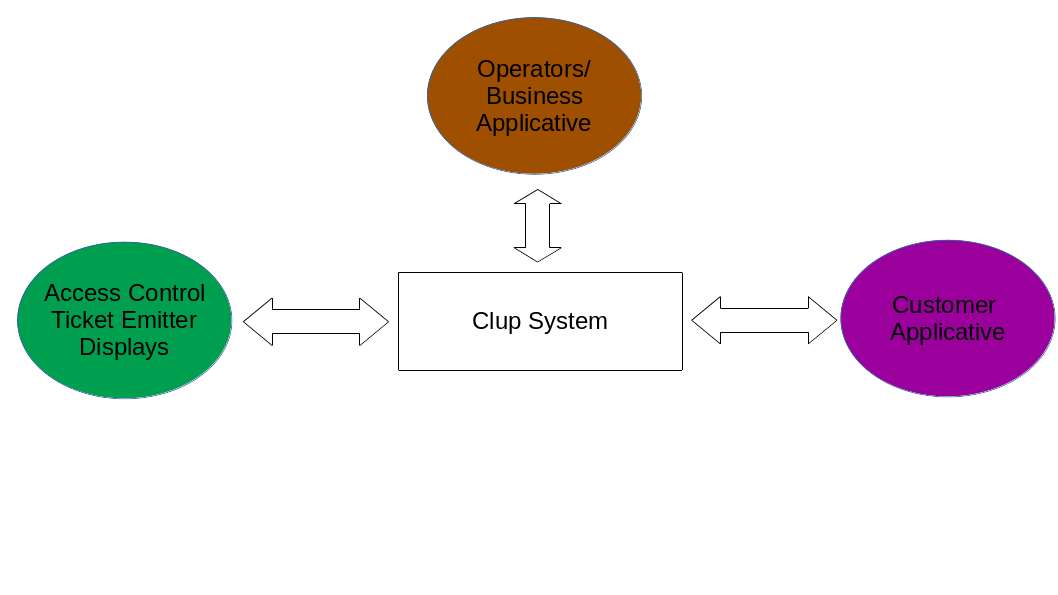
\includegraphics[width=\textwidth]{Images/system.png}
    \caption{\label{fig:Coarse_Grain_System}``The Machine'' and the components interfacing with ``The world''}
\end{figure}

\subsubsection{Shared phenomena}
%TODO: Probably to be relocated
Here is a list of shared phenomena happening in CLup
\begin{itemize}[label={}]
    \item SP1 The gate opens and lets the customer in the store (Machine Controlled)
    \item SP2 The customer scans his ticket at the gate (World Controlled)
    \item SP3 The customer leaves the store and their exit is counted by a people counting system (World Controlled)
    \item SP4 The customer books a ticket to enter the shop with the Customer Applicative (World Controlled)
    \item SP5 The customer receive a notification when the time to enter is near (Machine Controlled)
    \item SP6 The customer presses the button to request a paper tickets (World Controlled)
    \item SP7 The customer receives a ticket from the ticket printer and an estimated waiting time (Machine Controlled)
    \item SP8 The display at the entrance shows the next ticket called to enter (Machine Controlled)
\end{itemize}

\subsubsection{Interfacing with external systems}
The S2B have some interfaces with some other external system used to provide data to CLup 



\textbf{Physical ticket emitter} Not all users have CLup installed in their smartphones, to allow them to enter the store a paper ticket emitter is
placed near the entrance. The ticket emitter prints tickets in 
a paper support when a button is pressed. When the button is pressed the emitter connects to internet and via a dedicated API requests a new paper ticket number. The response will contain the needed information to print the ticket and the queue statistics in the system are updated accordingly. Optionally the emitter could have a mini screen where a waiting time estimation is shown.



A \textbf{Smart gate} is a composed of a mechanical actuator that opens and closes the gate, a QR code scanner and it is provided with connectivity to internet. When a QR code is scanned and decoded, a request is sent to the CLup API containing information about the ticket scanned.
The system checks the validity of the ticket and sends a response to the gate. If the response is affirmative the gate will open, if the scanned QR doesn't represent a valid ticket an error will be shown to the customer via visual and/or auditive feedbacks. Even if the gate replaces a big part of access control staff's work (see next paragraph), some human intervention could be required for security reasons, or to open the gate in exceptional cases. 


\textbf{People counters} located at shop exits counts people passing through that exit. They are connected to the network and will communicate the count of people that left the shop. This counter could be a turnstile or a sensor or even a QR scanner that scans same tickets used to enter, or a barcode printed in the receipt. CLup system works fine without them but these counter allow to have a precise count of the people inside the shop, and this datum could be useful to estimate more precisely the waiting times.

\textbf{Ticket number screens} are located ad the shop entrance. They display the latest ticket numbers called to the entrance and the next numbers up to enter.

\subsubsection{Interfacing with users}

\textbf{Access control operators} have a portable device equipped with a camera and internet connectivity. This device has the staff access control app installed on. The operator application user interface provides these functionalities:
\begin{itemize}
    \item Authenticate with a CLup operator account or corporation SSO service
    \item Check (and adjust) estimated occupancy of the whole shop and its departments
    \item Check length of the queues, and bookings in the time slots
    \item Scan a ticket qr code to allow a person to enter
    \item Notify the next customers in the virtual ticket queue alerting them to reach the entrance
\end{itemize}

\textbf{CLup Customer Application} provides an easy to use interface with these features:
\begin{itemize}
    \item Features available to all users:
    \begin{itemize}
        \item Create a new account 
        \item Login to an existing account
        \item Show a map of nearby store adopting CLup system and an option for listing them sorted by distance
        \item See real-time and projected occupancy of all stores
    \end{itemize}
    \item Features available to authenticated users:
    \begin{itemize}
        \item Create a virtual ticket to enter in a store immediately (if space is available) or when a space is available
        \item Check store occupancy in future time slots
        \item Book a visit to a store in a time slot (if space is available) 
    \end{itemize}
\end{itemize}

\subsection{Assumptions, dependencies and constraints}
\subsubsection{Domain Assumptions}
    \begin{itemize}[label={}]
        \item DA1 Customers that created a shoplist will buy approximately all the products in that list, so they will visit for the greater part of their permanence the departments where the products are located
        \item DA2 Customer will stay approximately the time they have declared when booking the ticket
        \item DA3 The access controller works properly and won't allow unauthorized customers entrances
        \item DA4 Customers with an in-place digital ticket try to avoid to stay near the entrance until they receive the ``go to entrance notification''
        \item DA5 Customers with a booked ticket in a given time slot will not show up until few minutes before the start of their time slots
        \item DA6 If a people counter is installed it will provide the exact count of the customer that left the shop
        \item DA7 No customer are present at the shop opening hour, and no costumer will be present at the shop closing hour
        \item DA8 The store manager will insert correct data about the shop and the departments maximum capacities
    \end{itemize}
\subsubsection{Dependencies}
\subsubsection{Constraints}

\subsection{Product Functions}    
    \begin{figure}
        \centering
        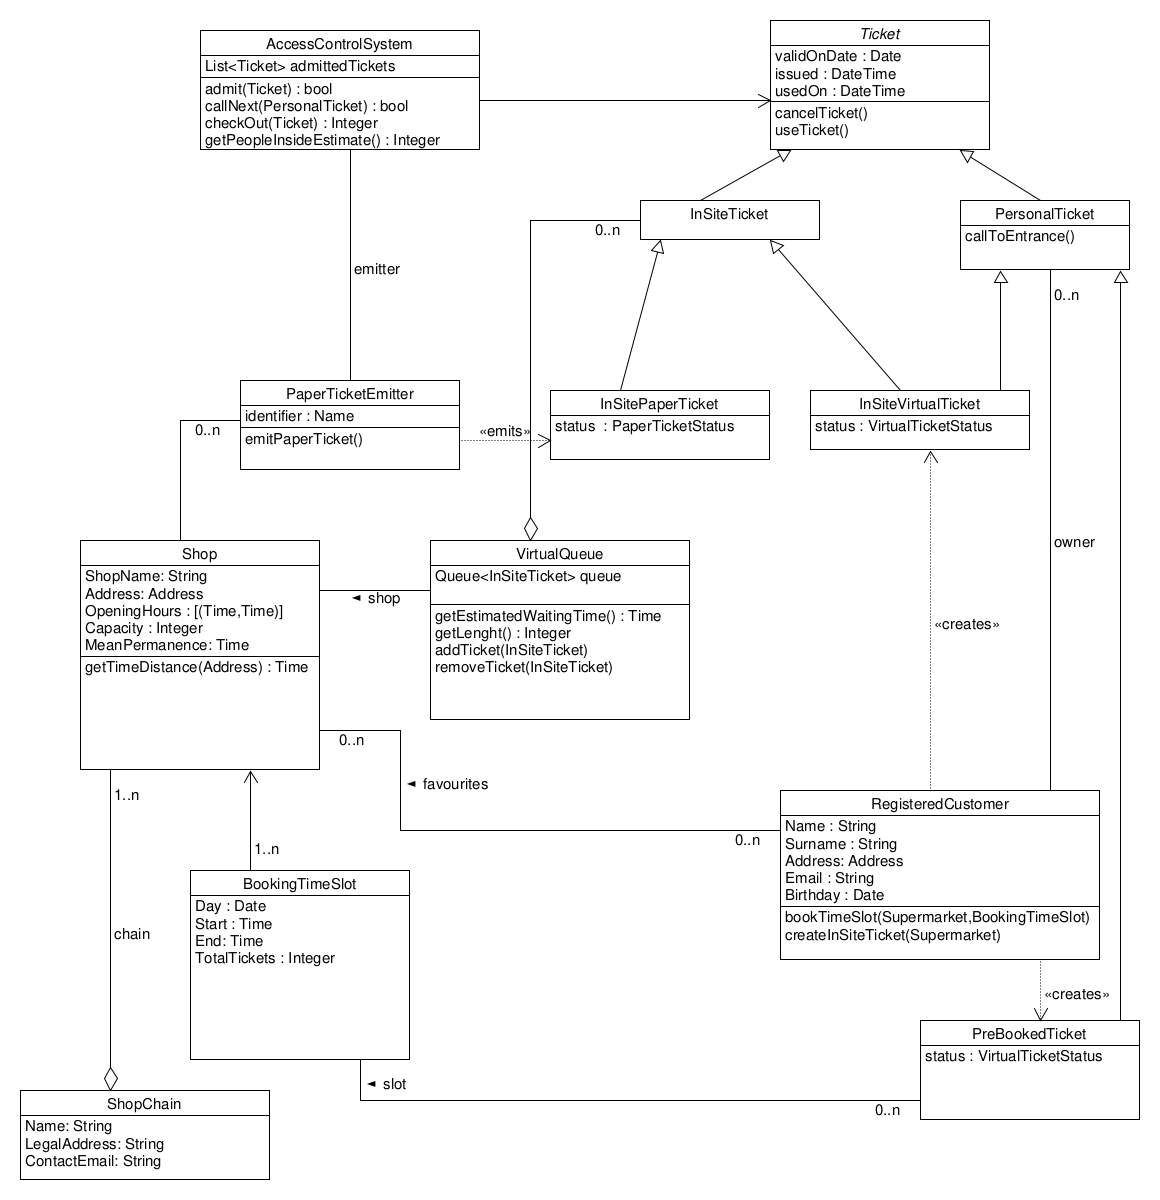
\includegraphics[width=\textwidth]{Images/UML_class_synthetic.png}
        \caption{\label{fig:Booked_Ticket_State}Class Diagram}
    \end{figure}
    \begin{figure}
    \centering
    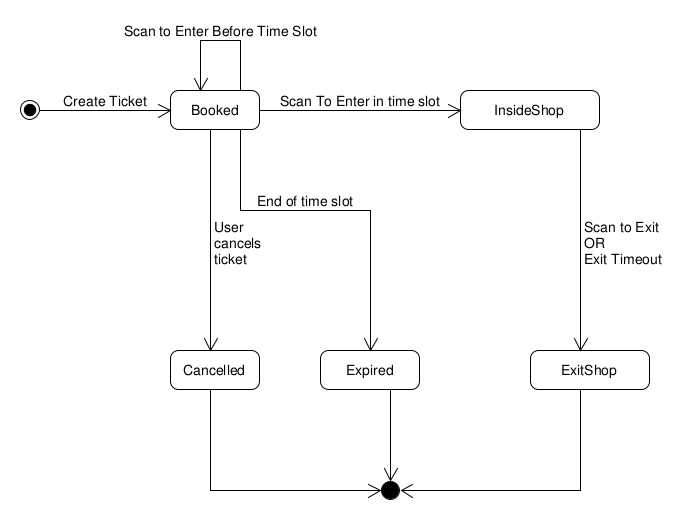
\includegraphics[width=\textwidth]{Images/UML_booked_ticket.png}
    \caption{\label{fig:Booked_Ticket_State}Booked ticket state machine}
    \end{figure}
    The state machines depicted in the state machines below (Figures n,n+1,n+2) show the different life cycles of the three possible tickets that allow customers to enter in the supermarkets: 
    \begin{figure}
        \centering
        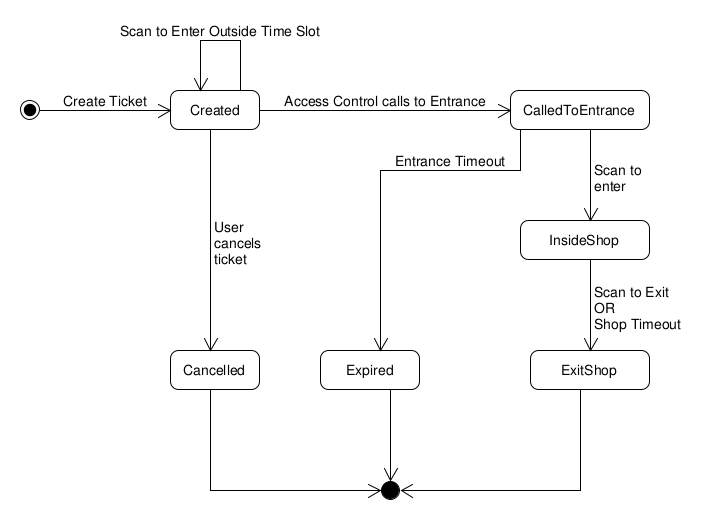
\includegraphics[width=\textwidth]{Images/UML_in_place_virtual_ticket.png}
        \caption{ \label{fig:Booked_Ticket_State}In place virtual ticket state machine}
    \end{figure}
    In the figure \ref{fig:Booked_Ticket_State} 
\subsection{User Characteristics}
    There are two macro-groups of people that will use CLup, the businesses adopting the system and the customers of these
    business using CLup to plan their visit to the shop.
    \subsubsection{Business-side Characteristics}
    CLup is addressed mainly to the big grocery shops, but could be used from every medium to big sized shop.
    CLup is very flexible, and will work in a lot of different scenarios, thanks to these features:
    \begin{itemize}
        \item Parameters of the system are tunable: The business could customize booking time slots duration and capacity
        \item Different access controls methods could be employed: The shop could install some smart gates with a QR scanner
              or could hire an employee that checks the tickets with a mobile device using the business CLup application. 
        \item Different precision levels of estimated data are possible, based on the data sources available:
              For example if the shop counts the number of people exiting the premises (using a turnstile or a QR scanner) 
              CLup will provide the exact occupancy, but if this is not possible an estimation will be provided, based on the 
              average permanence time in the shop.  
          
    \end{itemize}
    \subsubsection{Customer side characteristics}
    All the people need to do grocery shopping especially during the lockdown measures enacted due to COVID-19. 
    Every one should be able to access the shop, even the people that can't download the CLup application.
    The S2B solves this problem by allowing the customer a paper ticket and wait in a physical line before entering the shop if the shop is full.
    The physical line of customer is unavoidable if the supermarket could not satisfy the increased demand of groceries in its catching area, even if CLup could alleviate this problem allowing to better distribute the customer visits during the shop opening hours. The possibility of booking the visit in advance will push more and more users to download CLup to avoid the queue, and be safer avoiding to cram at the entrance.




%------------------------------------------------------------------------------------------------------------------------------------------------
\clearpage
\section{Specific Requirements}
\label{sect:requirements}
\subsection{External Interface Requirements}
\subsubsection{User Interfaces}
\subsubsection{Hardware Interfaces}
\subsubsection{Software Interfaces}
\subsubsection{Communication Interfaces}
\subsection{Functional Requirements}
\subsubsection{Use cases}
Here is a list of relevant use cases for the S2B
\smallskip

\rowcolors{2}{gray!25}{white}
\renewcommand{\arraystretch}{1.4}
\begin{tabular}{C{2cm}L{10.5cm}C{2.6cm}}
    \rowcolor{gray!50}
    Label & Use Case                                                                                         \\
    UC1   & Customer Registration                                                                            \\
    UC2   & Customer Authentication                                                                          \\
    UC3   & Customer search for the store page                                                               \\
    UC4   & Customer adds/removes a store to their favorites list                                            \\
    UC5   & Customer books a visit in a store                                                                \\
    UC6   & Customer creates/edits a shopping list                                                           \\
    UC7   & Customer create a numbered virtual ticket to enter a store as soon as there is a place available \\
    UC8   & Customer creates a physical numbered ticket                                                      \\
    UC9   & Customer cancels a previously created ticket                                                     \\
    UC10  & Customer scans the ticket in an access control system to enter                                   \\
    UC11  & An user leaves the store through an exit with a people counter installed                         \\
    UC12  & A store operator checks statistics about the store                                               \\
\end{tabular}


\medskip
\clearpage
% COuld be useful to report this on the dictionary section on chapter 1%
In the following use case description tables, if not explicitly stated otherwise, the term ``user'' is used interchangeably with the term customer ``customer''.
\medskip

\textbf{Use case 1: User Registration}
\smallskip

\rowcolors{1}{white}{white}
\begin{longtable}{p{0.25\linewidth}p{0.75\linewidth}}
    \toprule
    \textbf{Name}             & \textbf{User Registration}                                                                                                        \\
    \midrule
    \textbf{Actors}           & Unregistered customer                                                                                                             \\
    \midrule
    \textbf{Entry conditions} & The user requests the system to register                                                                                          \\
    \midrule
    \textbf{Flow of events}   &
    \begin{enumerate}
        \item The system shows the form with the required fields to register
        \item The user inserts his e-mail address and his password
        \item The user inserts his name, surname, birth date and his preferred home address
        \item The user is shown the recap of the information used to fill the form
        \item The user confirms the information, and the form is sent to the system
        \item The system sends a e-mail to the address provided by the user in the form. The e-mail contains a verification link
        \item The users open the e-mail and clicks on the verification link
        \item The system sends an e-mail to the user stating that their registration process ended successfully
    \end{enumerate}                                                                                                                                     \\
    \midrule
    \textbf{Exit conditions}  & The unregistered customer now is a registered customer and after authenticating could access to all CLup customer functionalities \\
    \midrule
    \textbf{Exceptions}       &
    \begin{itemize}
        \item If the email inserted is already registered in the system an error message is prompted asking the user to insert another e-mail address
        \item If the password doesn't meet the safety requirements an error message is prompted showing the requirements for the password and asking the user to insert a new safe password
    \end{itemize}                                                                                                                                     \\
    \bottomrule
    \caption{\emph{Customer registration} use case description}
\end{longtable}


\clearpage
\textbf{Use case 2: User Authentication}
\smallskip
\rowcolors{1}{white}{white}
\begin{longtable}{p{0.25\linewidth}p{0.75\linewidth}}
    \toprule
    \textbf{Name}             & \textbf{User Authentication}                                                                                 \\
    \midrule
    \textbf{Actors}           & Registered Customer                                                                                          \\
    \midrule
    \textbf{Entry conditions} & The user requests the system to log-in                                                                       \\
    \midrule
    \textbf{Flow of events}   &
    \begin{enumerate}
        \item The system shows the authentication form
        \item The user fills the form with his e-mail address used to register and his password
        \item The system checks if there exists one account registered with the provided e-mail
        \item The system checks that the account's password matches with the one that is provided in the form
        \item The initial CLup page is shown to the user
    \end{enumerate}                                                                                                                \\
    \midrule
    \textbf{Exit conditions}  & The unregistered customer now is a registered customer and could access to all CLup customer functionalities \\
    \midrule
    \textbf{Exceptions}       &
    \begin{itemize}
        \item If the email or the password are incorrect then then an error message is shown to the user
    \end{itemize}                                                                                                                \\
    \bottomrule
    \caption{\emph{Customer authentication} use case description}
\end{longtable}

\clearpage
\textbf{Use case 3: Customer searches for store details}
\smallskip
\rowcolors{1}{white}{white}
\begin{longtable}{p{0.25\linewidth}p{0.75\linewidth}}
    \toprule
    \textbf{Name}                             & \textbf{Customer searches for store details}      \\
    \midrule
    \textbf{Actors}                           & Customer                                          \\
    \midrule
    \textbf{Entry conditions}                 & The user started the CLup customer application    \\
    \midrule
    \textbf{Flow of events}                   &
    \begin{enumerate}
        \item The system checks the position of the user with the GPS
        \item The system interfaces with an external map API downloading from it a map of the surroundings of the user position
        \item The system decorates the map with the positions of all supermarkets adopting CLup
        \item The system sends the map to the user
        \item The user applies filters on the store list
        \item The system updates the map displaying only the stores complying with the filter
        \item The user selects one store
        \item The system retrieves all the details about the store from his databases
        \item The system loads and displays the store view
    \end{enumerate}                                                                     \\
    \midrule
    \textbf{Exit conditions}                  & The customer now views the store pages and could:
    \begin{itemize}
        \item \textbf{book a visit in that store}
        \item \textbf{create a numbered ticket for entering the store as soon as possible}
        \item \textbf{add the store to their favorites list}
    \end{itemize}                                                                     \\
    \midrule
    \textbf{Exceptions}                       &
    \begin{itemize}
        \item If the GPS position is not available or the user doesn't want to provide it to the system, the system will center the map view at the user's home address specified in the registration, making a call to a Geocoding API to retrieve home coordinates
        \item If the Geocoding API call fails or returns no result the map will be centered to the last known user position
        \item If the Map API call fails or there isn't a last known position a default list view containing all CLup stores will be shown to the user
        \item If no store matches the user filters an error message will be prompted to the user
    \end{itemize}                                                                     \\
    \midrule
    \textbf{Additional \newline Requirements} &
    \begin{itemize}
        \item The store details shown in the store view are Store name, store chain, address, opening hour, occupancy statistics at every hour
        \item The filters criteria available to the user are: Store name, city, currently open stores, maximum distance from the store
    \end{itemize}                                                                     \\
    \bottomrule
    \caption{\emph{Customer searches for store details} use case description}
\end{longtable}

\clearpage
\textbf{Use case 4: Customer adds/removes a store to their favorites list}
\smallskip
\rowcolors{1}{white}{white}
\begin{longtable}{p{0.25\linewidth}p{0.75\linewidth}}
    \toprule
    \textbf{Name}             & \textbf{Customer adds/removes a store to their favorites list} \\
    \midrule
    \textbf{Actors}           & Registered customer                                            \\
    \midrule
    \textbf{Entry conditions} & The user is authenticated and has loaded a store view          \\
    \midrule
    \textbf{Flow of events}   &
    \begin{enumerate}
        \item The user clicks on the button to add/remove the store from the favorites
        \item If the store is on the user's favorites list the store is removed from that list else the store is added to that list
    \end{enumerate}                                                                 \\
    \midrule
    \textbf{Exit conditions}  & The user sees the change on their favourite list               \\
    \midrule
    \textbf{Exceptions}       &                                                                \\
    \bottomrule
    \caption{\emph{Customer adds/removes a store to their favorites list} use case description}
\end{longtable}


\clearpage
\textbf{Use case 5: Customer books a visit in a store}
\smallskip
\rowcolors{1}{white}{white}
\begin{longtable}{p{0.25\linewidth}p{0.75\linewidth}}
    \toprule
    \textbf{Name}             & \textbf{Customer books a visit in a store}                                                           \\
    \midrule
    \textbf{Actors}           & Registered customer                                                                                  \\
    \midrule
    \textbf{Entry conditions} & The user is authenticated and has loaded a store view. The user has no other visits or ticket active \\
    \midrule
    \textbf{Flow of events}   &
    \begin{enumerate}
        \item The user starts the procedure selecting the option to book a visit from the store page
        \item The user selects a date
        \item The system retrieves the time slots with at least one free bookable slot and shows them to the user
        \item The user selects his preferred slots sending the information to the System
        \item The systems asks the user to select the expected duration of his visit, showing to them a default value
        \item The user (optionally) edits the value and then confirm the booking
        \item The system confirms the booking of the visit
        \item The system asks the customer if they want to \textbf{create a shopping list}
    \end{enumerate}                                                                                                       \\
    \midrule
    \textbf{Exit conditions}  & The user could enter the store during the booked time-slot                                           \\
    \midrule
    \textbf{Exceptions}       &                                                                                                      \\
    \bottomrule
    \caption{\emph{Customer books a visit in a store} use case description}
\end{longtable}

\clearpage
\textbf{Use case 6: Customer creates/edits a shopping list}
\smallskip
\rowcolors{1}{white}{white}
\begin{longtable}{p{0.25\linewidth}p{0.75\linewidth}}
    \toprule
    \textbf{Name}             & \textbf{Customer creates/edits a shopping list} \\
    \midrule
    \textbf{Actors}           & Registered customer                             \\
    \midrule
    \textbf{Entry conditions} & The user is authenticated                       \\
    \midrule
    \textbf{Flow of events}   &
    \begin{enumerate}
        \item The user reaches the shopping list view
        \item If the user added a shopping list before, the system asks the user if they want to edit the old list or if they want to start from a blank one
        \item The user inputs a search key in a search bar
        \item The system searches products matching the key and shows them ordered by closeness to the search key
        \item The user choses zero or more than one product from the search results and adds to the shopping list
        \item The user views the complete shopping list and could continue adding products or removing them until it accepts the list.
        \item When the user confirms the list, the system will save it in order to make it available to the user the next time they want to compile a shopping list
        \item If the user has booked a visit the system can update the estimates on store departments occupancy on the time of the visit thanks the data on the shopping list
        \item The system acknowledges the user that the list has been saved
    \end{enumerate}                                                  \\
    \midrule
    \textbf{Exit conditions}  &                                                 \\
    \midrule
    \textbf{Exceptions}       &                                                 \\
    \bottomrule
    \caption{\emph{Customer creates/edits a shopping list} use case description}
\end{longtable}

\clearpage
\textbf{Use case 7: Customer create a numbered virtual ticket to enter a store as soon as there is place available}
\smallskip
\rowcolors{1}{white}{white}
\begin{longtable}{p{0.25\linewidth}p{0.75\linewidth}}
    \toprule
    \textbf{Name}             & \textbf{Customer create a numbered virtual ticket to enter a store as soon as there is place available} \\
    \midrule
    \textbf{Actors}           & Registered customer                                                                                     \\
    \midrule
    \textbf{Entry conditions} & The user is authenticated and has loaded a store view. The user has no other visits or ticket active    \\
    \midrule
    \textbf{Flow of events}   &
    \begin{enumerate}
        \item The user starts the procedure selecting the option to retrieve a numbered ticket from the store page
        \item The system estimates the waiting time based on the number of people queued and the people actually inside the store
        \item The system confirms the emission of the ticket to the user and shows them the number and other ticket details
        \item If the waiting time changes in a significant way the system notifies the user with the new waiting time
        \item The system alerts the user when it's time to approach the entrance
    \end{enumerate}                                                                                                          \\
    \midrule
    \textbf{Exit conditions}  & The user goes to the entrance and scans the ticket                                                      \\
    \midrule
    \textbf{Exceptions}       &
    \begin{itemize}
        \item If the waiting time is long the system shows an alert to the user asking if they are sure of creating the ticket despite the long queue
        \item If the user takes too long to enter the supermarket after being called to enter an alert is shown stating that the entry is no more guaranteed with that ticket

    \end{itemize}                                                                                                          \\
    \bottomrule
    \caption{\emph{Customer creates a numbered ticket to enter a store as soon as there is place available} use case description}
\end{longtable}

\clearpage
\textbf{Use case 8: Customer create a numbered physical ticket to enter the store}
\smallskip
\rowcolors{1}{white}{white}
\begin{longtable}{p{0.25\linewidth}p{0.75\linewidth}}
    \toprule
    \textbf{Name}             & \textbf{Customer create a numbered physical ticket to enter the store}                                                                   \\
    \midrule
    \textbf{Actors}           & Customer, Physical Ticket Emitter                                                                                                        \\
    \midrule
    \textbf{Entry conditions} & The customer is in front of the ticket emitter                                                                                           \\
    \midrule
    \textbf{Flow of events}   &
    \begin{enumerate}
        \item The user selects a button to create a new ticket
        \item The emitter request the system to create a new numbered ticket
        \item The system estimates the waiting time based on the number of people queued and the people actually inside the store
        \item The system returns the details of the ticket to the emitter
        \item The emitter prints the ticket
        \item The user retrieves the ticket and waits until the number on his ticket is called at the entrance of the store
    \end{enumerate}                                                                                                                                           \\
    \midrule
    \textbf{Exit conditions}  & The user enters the store scanning the ticket                                                                                            \\
    \midrule
    \textbf{Exceptions}       & If the user takes too long to enter the supermarket after being called to enter, the ticket no more guarantees the entrance to the store \\
    \bottomrule
    \caption{\emph{Customer create a numbered physical ticket to enter the store} use case description}
\end{longtable}

\clearpage
\textbf{Use case 9: Customer cancels a previously created ticket}
\smallskip
\rowcolors{1}{white}{white}
\begin{longtable}{p{0.25\linewidth}p{0.75\linewidth}}
    \toprule
    \textbf{Name}             & \textbf{Customer cancels a previously created ticket}          \\
    \midrule
    \textbf{Actors}           & Registered Customer                                            \\
    \midrule
    \textbf{Entry conditions} & The customer has a visit to a store booked or a                \\
    \midrule
    \textbf{Flow of events}   &
    \begin{enumerate}
        \item The customer from the virtual ticket/booking view selects the option to cancel the ticket/booking
        \item The system deletes the item from the database and triggers a reevaluation of the estimations about the occupancy of the store and the departments
        \item The system acknowledges the user that the operation was successful
    \end{enumerate}                                                                 \\
    \midrule
    \textbf{Exit conditions}  & The user could now create another ticket or book another visit \\
    \midrule
    \textbf{Exceptions}       &                                                                \\
    \bottomrule
    \caption{\emph{Customer cancels a previously created ticket} use case description}
\end{longtable}

\clearpage
\textbf{Use case 10: Customer scans the ticket on an access control system to enter the store}
\smallskip
\rowcolors{1}{white}{white}
\begin{longtable}{p{0.25\linewidth}p{0.75\linewidth}}
    \toprule
    \textbf{Name}                               & \textbf{Customer scans the ticket on an access control system to enter the store} \\
    \midrule
    \textbf{Actors}                             & Customer, Access Control System                                                   \\
    \midrule
    \textbf{Entry conditions}                   & The customer has a ticket or a visit reservation                                  \\
    \midrule
    \textbf{Flow of events}                     &
    \begin{enumerate}
        \item The user scans the machine readable identifier of the ticket on the access control system
        \item The access control system sends the scanned ticket identifier to the system
        \item The system determines if the customer can enter, retrieving information about the ticket and the current occupancy of the supermarket
        \item The system sends a confirm to the Access Control System
        \item The Access Control System lets the customer enter
    \end{enumerate}                                                                                                      \\
    \midrule
    \textbf{Exit conditions}                    & The user is inside the store                                                      \\
    \midrule
    \textbf{Exceptions}                         &
    \begin{itemize}
        \item If the access control system fails to recognize the ticket identifer, the user will be asked to scan again the ticket
        \item If the ticket is not valid, the Access Control System won't let the customer enter. This decision could be overridden by an human operator if the system is manned
        \item If the supermarket occupancy is over the legal capacity, the access control won't let the customer enter even with a valid ticket. The system will ask the customer to wait and will consider the booking of the current time slot valid also after the expiration
        \item If the access control system fails to communicate to the system, the customer is asked to scan again the ticket and if fails again asks the customer to notify the store personnel (only if the system is not manned).
    \end{itemize}                                                                                                      \\
    \bottomrule
    \textbf{Additional \linebreak Requirements} &
    \begin{itemize}
        \item A booked ticket is valid only in the booked date within the time slot indicated in the ticket.
        \item A numbered ticket is valid only for a limited time after the ticket number has been called to the entrance.
        \item All the tickets are bound to a specific store and could be used only on that store.
        \item The store could let enter customer with an expired ticket if the store is far to being full.
    \end{itemize}                                                                                                      \\
    \bottomrule
    \caption{\emph{Customer scans the ticket in an access control system to enter the store} use case description}
\end{longtable}

\clearpage
\textbf{Use case 11: An user leaves the store through an exit with a people counter installed}
\smallskip
\rowcolors{1}{white}{white}
\begin{longtable}{p{0.25\linewidth}p{0.75\linewidth}}
    \toprule
    \textbf{Name}             & \textbf{An user leaves the store through an exit with a people counter installed}    \\
    \midrule
    \textbf{Actors}           & Customer, People Counter                                                             \\
    \midrule
    \textbf{Entry conditions} & The customer is inside the store                                                     \\
    \midrule
    \textbf{Flow of events}   &
    \begin{enumerate}
        \item The customer walks out of the store through a gate with a people counter installed
        \item The people counter registers that a person passed through the gate
        \item The people counter contacts the system, updating the occupancy real time information
    \end{enumerate}                                                                                       \\
    \midrule
    \textbf{Exit conditions}  & The customer is out of the store and the count of the people of the store is updated \\
    \midrule
    \textbf{Exceptions}       &                                                                                      \\
    \bottomrule
    \caption{\emph{An user exits the store through an exit with a people counter installed} use case description}
\end{longtable}

\clearpage
\textbf{Use case 12: A store operator checks statistics about the store}
\smallskip
\rowcolors{1}{white}{white}
\begin{longtable}{p{0.25\linewidth}p{0.75\linewidth}}
    \toprule
    \textbf{Name}             & \textbf{A store operator checks statistics about the store}                                        \\
    \midrule
    \textbf{Actors}           & Store Operator/ Store Manager                                                                      \\
    \midrule
    \textbf{Entry conditions} & The Store Operator/Store Manager is authenticated                                                  \\
    \midrule
    \textbf{Flow of events}   &
    \begin{enumerate}
        \item The store operator requires to see a statistic or real time information about the store collected with CLup
        \item The system retrieves or compute that information
        \item The system present the data to the Operator/Manager
    \end{enumerate}                                                                                                     \\
    \midrule
    \textbf{Exit conditions}  & The Operator/System now can see the data presented by the System                                   \\
    \midrule
    \textbf{Exceptions}       & The system throws an error to the operator if he has no privilege to see the requested information \\
    \bottomrule
    \caption{\emph{A store operator checks statistics about the store} use case description}
\end{longtable}


\subsubsection{Requirements Mapping}
\subsection{Performance Requirements}
Regarding the \textbf{CLup customer application} and the \textbf{CLup customer operator}  an user input that triggers an action that requires the communication with a remote server should take no longer than 5 seconds, from the start of the interaction to the moment when the user receives some feedback. When the user input doesn't trigger actions that need the communication with a remote server this time should be lower than 1 second. This requirements holds in a context where the underlying operative system is not overloaded and the user internet connection is working properly.
\smallskip
When a store admin account request elaborate statistics regarding the store the response time must be lower than 10 seconds.
\subsection{Design Constraints}
\subsection{Software System Attributes}
\subsubsection{Reliability}
All the data stored in the CLup databases must be periodically backed up. Data redundancy policies, like RAID, must be enacted for handling failures promptly and lowering the risk of losing data.

\subsubsection{Availability}
The system must have multiple nodes handling requests from the customers and the operators. These nodes, working in parallel reduce the risk of a total failure of the system. Data redundancy policies also help to reduce downtimes in case of a data storage unit fault.

\smallskip

The system uptime should be closer to the 100\% as possible. Since that is impossible an uptime of 99.9\% is more than acceptable and corresponds to less than 9 hours of down time every 365 days.
Ordinary maintenance that needs shutting down part of the system should be planned, if possible, during nights in this way is more likely that the majority of the users don't experience disruptions in the CLup services.

\smallskip

The access control system must continue working even if an external system installed in the supermarket fails. In the following table are listed the measures that must be taken after a failure of an external system
\smallskip

\rowcolors{2}{gray!25}{white}
\begin{tabular}{C{5cm}L{10.0cm}C{2.0cm}}
    \rowcolor{gray!50}
    External System that fails & Measures                                                                                                                                   \\
    People counter             & The CLup system will estimate the number of people inside the store using the mean visit times. This value could also be adjusted manually \\
    Smart Gates                & An operator with the CLup operator application could check tickets and admit people manually                                               \\
    Paper Ticket Emitter       & An operator forms a queue and admits people manually if there is space in the store                                                        \\
    Ticket number screens      & An operator announces manually the ticket number called to enter the store seeing them on the operator application                         \\
\end{tabular}
\subsubsection{Security}
All the data sent via a insecure communication channels (i.e. Internet, Local Networks) must be secured with modern encryption standards. This requirement applies to all data exchanged from CLup customer and operator applications and for all traffic generated from the external hardware systems installed on the supermarket.

\smallskip

The external hardware systems installed in the supermarket should be connected in a secure and dedicated LAN with a single access point to the internet with the proper firewall settings. This network must be separated from other networks especially the ones accessible freely from the customers (i.e. a shop free wi-fi service).

\smallskip

The customer accounts are separated from the business accounts. Each store manager has the permission to manage the operator accounts and has access to all the store data, and could decide which account could view which statistics.
\subsubsection{Maintainability}
The system is clearly divided in a lot of independent subsystems that communicate between them using some interfaces. As long as the interface is not changed is possible to maintain and update the single subsystems without having to change the other subsystems
\subsubsection{Portability}
\textbf{The CLup customer mobile application} compatibility should cover the 95\% of the iOS and Android devices. To make CLup even more accessible a mobile friendly web interface must be provided to the user.

\smallskip

\textbf{The CLup operator application} must be available via a web application, and functionality needed from the Access Control Staff must be available in a mobile application to install in the devices given to the staff.
\subsection{Other Requirements}
\subsubsection{Required fields for registration}
When a CLup customer creates a CLup customer account, they have to fill a form. Here are specified requirements regarding the information needed to register to CLup. If not otherwise specified every field is compulsory.

\begin{itemize}
    \item First name
    \item Last name
    \item Address, composed of:
          \begin{itemize}
              \item Country
              \item Region/State
              \item Town
              \item CAP
              \item Street and number
              \item Additional address lines (optional)
          \end{itemize}
    \item Gender (optional)
    \item Date of birth
    \item Valid email address
    \item Password, must respect this criteria:
          \begin{itemize}
              \item Must have at least a digit
              \item Must have at least a lowercase character
              \item Must have at least a special symbol in this list
                    \begin{verbatim}
            *.!@#$%^&(){}[]:;<>,.?/~_+-=|\
        \end{verbatim}
              \item Must have a number of character between 8 and 32
          \end{itemize}
\end{itemize}

%------------------------------------------------------------------------------------------------------------------------------------------------
\clearpage
\section{Formal Analysis Using Alloy}
\label{sect:alloy}
A model written using a modeling language like Alloy is useful to understand better the problem and to check if the modeling of the problem is correct or needs to be refined. Alloy generates some instances starting from the model code in order to catch modeling errors. Fixing these errors in the early stages of the system lifecycle will cost a lot less than fixing them at later stages of the development cycle.

\subsection{Goals of the model}
The Alloy model proposed in the next subsection of this document will focus on the formalization of the queueing of the customers and the slot booking system. This model is static, meaning that each instance generated from the alloy engine depicts the state of the system in a given instant of the time. The goal of a static model is to generate instances from that model, these instances represent only the states that the system could assume the transition between these state are instead described from a dynamic model. Finding an invalid state means that something is wrong in the system or in the model, but if all states analyzed are correct this will not mean that the system static model is correct.
\subsection{Alloy Code}

\lstinputlisting[language=alloy]{alloy/model.als}
\clearpage
\subsection{Instance Analysis}
In this section some instances generated from the alloy engine will be shown in order to explain better the model.
For clarity some atoms and some relations between them are hidden. 
\begin{figure}[H]
    \hspace*{3.0cm}
    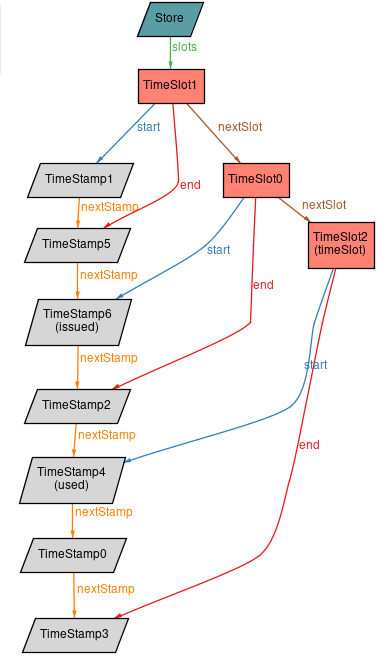
\includegraphics[scale=1.0]{Images/alloy_1_slots.png}
    \caption{\label{fig:Alloy_1}Instance diagram showing the Time Slots}
\end{figure}    

As shown in the Figure~\ref{fig:Alloy_1} the continuos time is modeled using discrete ordered timestamps. A timestamp is an instant of time when something relevant for the system happens (i.e. a time slot starts, a ticket is issued or used to enter the store). Each instance offers a view of a valid system state at the last (largest) timestamp, that in the first instance is TimeStamp0.

\pagebreak

In the Figure~\ref{fig:Alloy_1} instance diagram time slots atoms are shown. Every couple of time slots created from the same store must not overlap and the next time slot should start after the end of the current one.


\begin{figure}[H]
    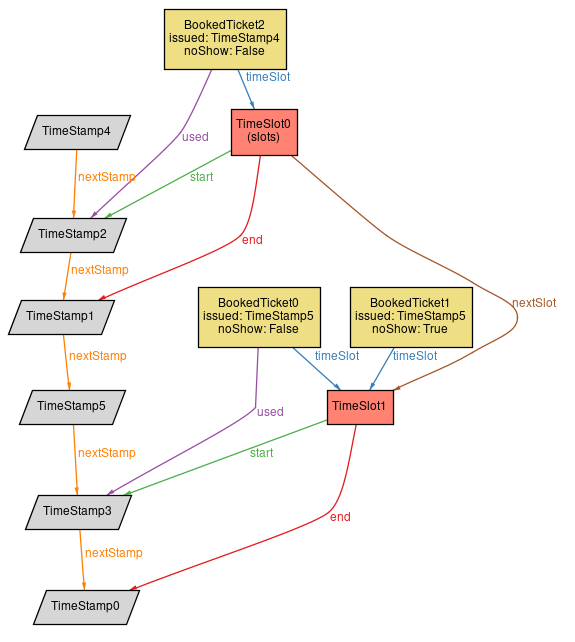
\includegraphics[width=\textwidth]{Images/alloy_3_booked.png}
    \caption{\label{fig:Alloy_2}Instance diagram showing Booked Tickets}
\end{figure}
In the Figure~\ref{fig:Alloy_2} booked tickets are shown in the diagram. Booked Tickets are a special type of ticket that are bound to a time slot. A Booked Ticket must be issued before the start of the time slot, and it has to be used within its time slot. A Booked Ticket not used in the bounded TimeSlots counts as a no-show ticket (representing the customer that books a ticket but does not show to the store in time).

\begin{figure}[H]
    \hspace*{2.8cm}
    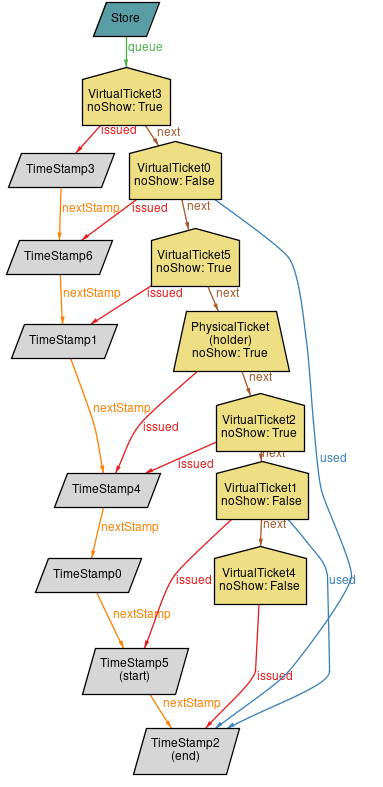
\includegraphics[]{Images/alloy_2_queue.png}
    \caption{\label{fig:Alloy_3}Instance diagram showing the queueing system}
\end{figure}

The Figure~\ref{fig:Alloy_3} explains how the store queueing system is modeled. If a customer doesn't book a ticket for entering in the store they have to retrieve a Numbered Ticket, either Virtual (using the application) or Physical (using the ticket emitter). These tickets are handed using a First Come First Served Logic, a ticket with a lower timestamp should be called to the entrance before a ticket with an higher one, and the timestamp when the ticket is used should reflect this order unless no-shows happen (i.e. A Customer that retrieves a ticket and then does not show when called to the entrance).

%------------------------------------------------------------------------------------------------------------------------------------------------
\clearpage
\section{Effort Spent}
\label{sect:effort}
Provide here information about how much effort each group member spent in working at this document. We would appreciate details here.



%------------------------------------------------------------------------------------------------------------------------------------------------
\clearpage
\addcontentsline{toc}{section}{References}
\bibliographystyle{plain}
\bibliography{main}
%------------------------------------------------------------------------------------------------------------------------------------------------




\end{document}
